% !TEX root = thesis.tex

\documentclass[thesis.tex]{subfiles}

\begin{document}

\chapter{Camera Module}
\label{appendix:camera-module}

The camera module photographed from the top and side. Cardboard is used to encase the taggant and cover it from ambient lighting. An additional piece of cardboard is used to set the smartphone to be at a fixed distance (of lens MFD) from the taggant allowing more accurate focus.

\begin{figure}[h]
\centering 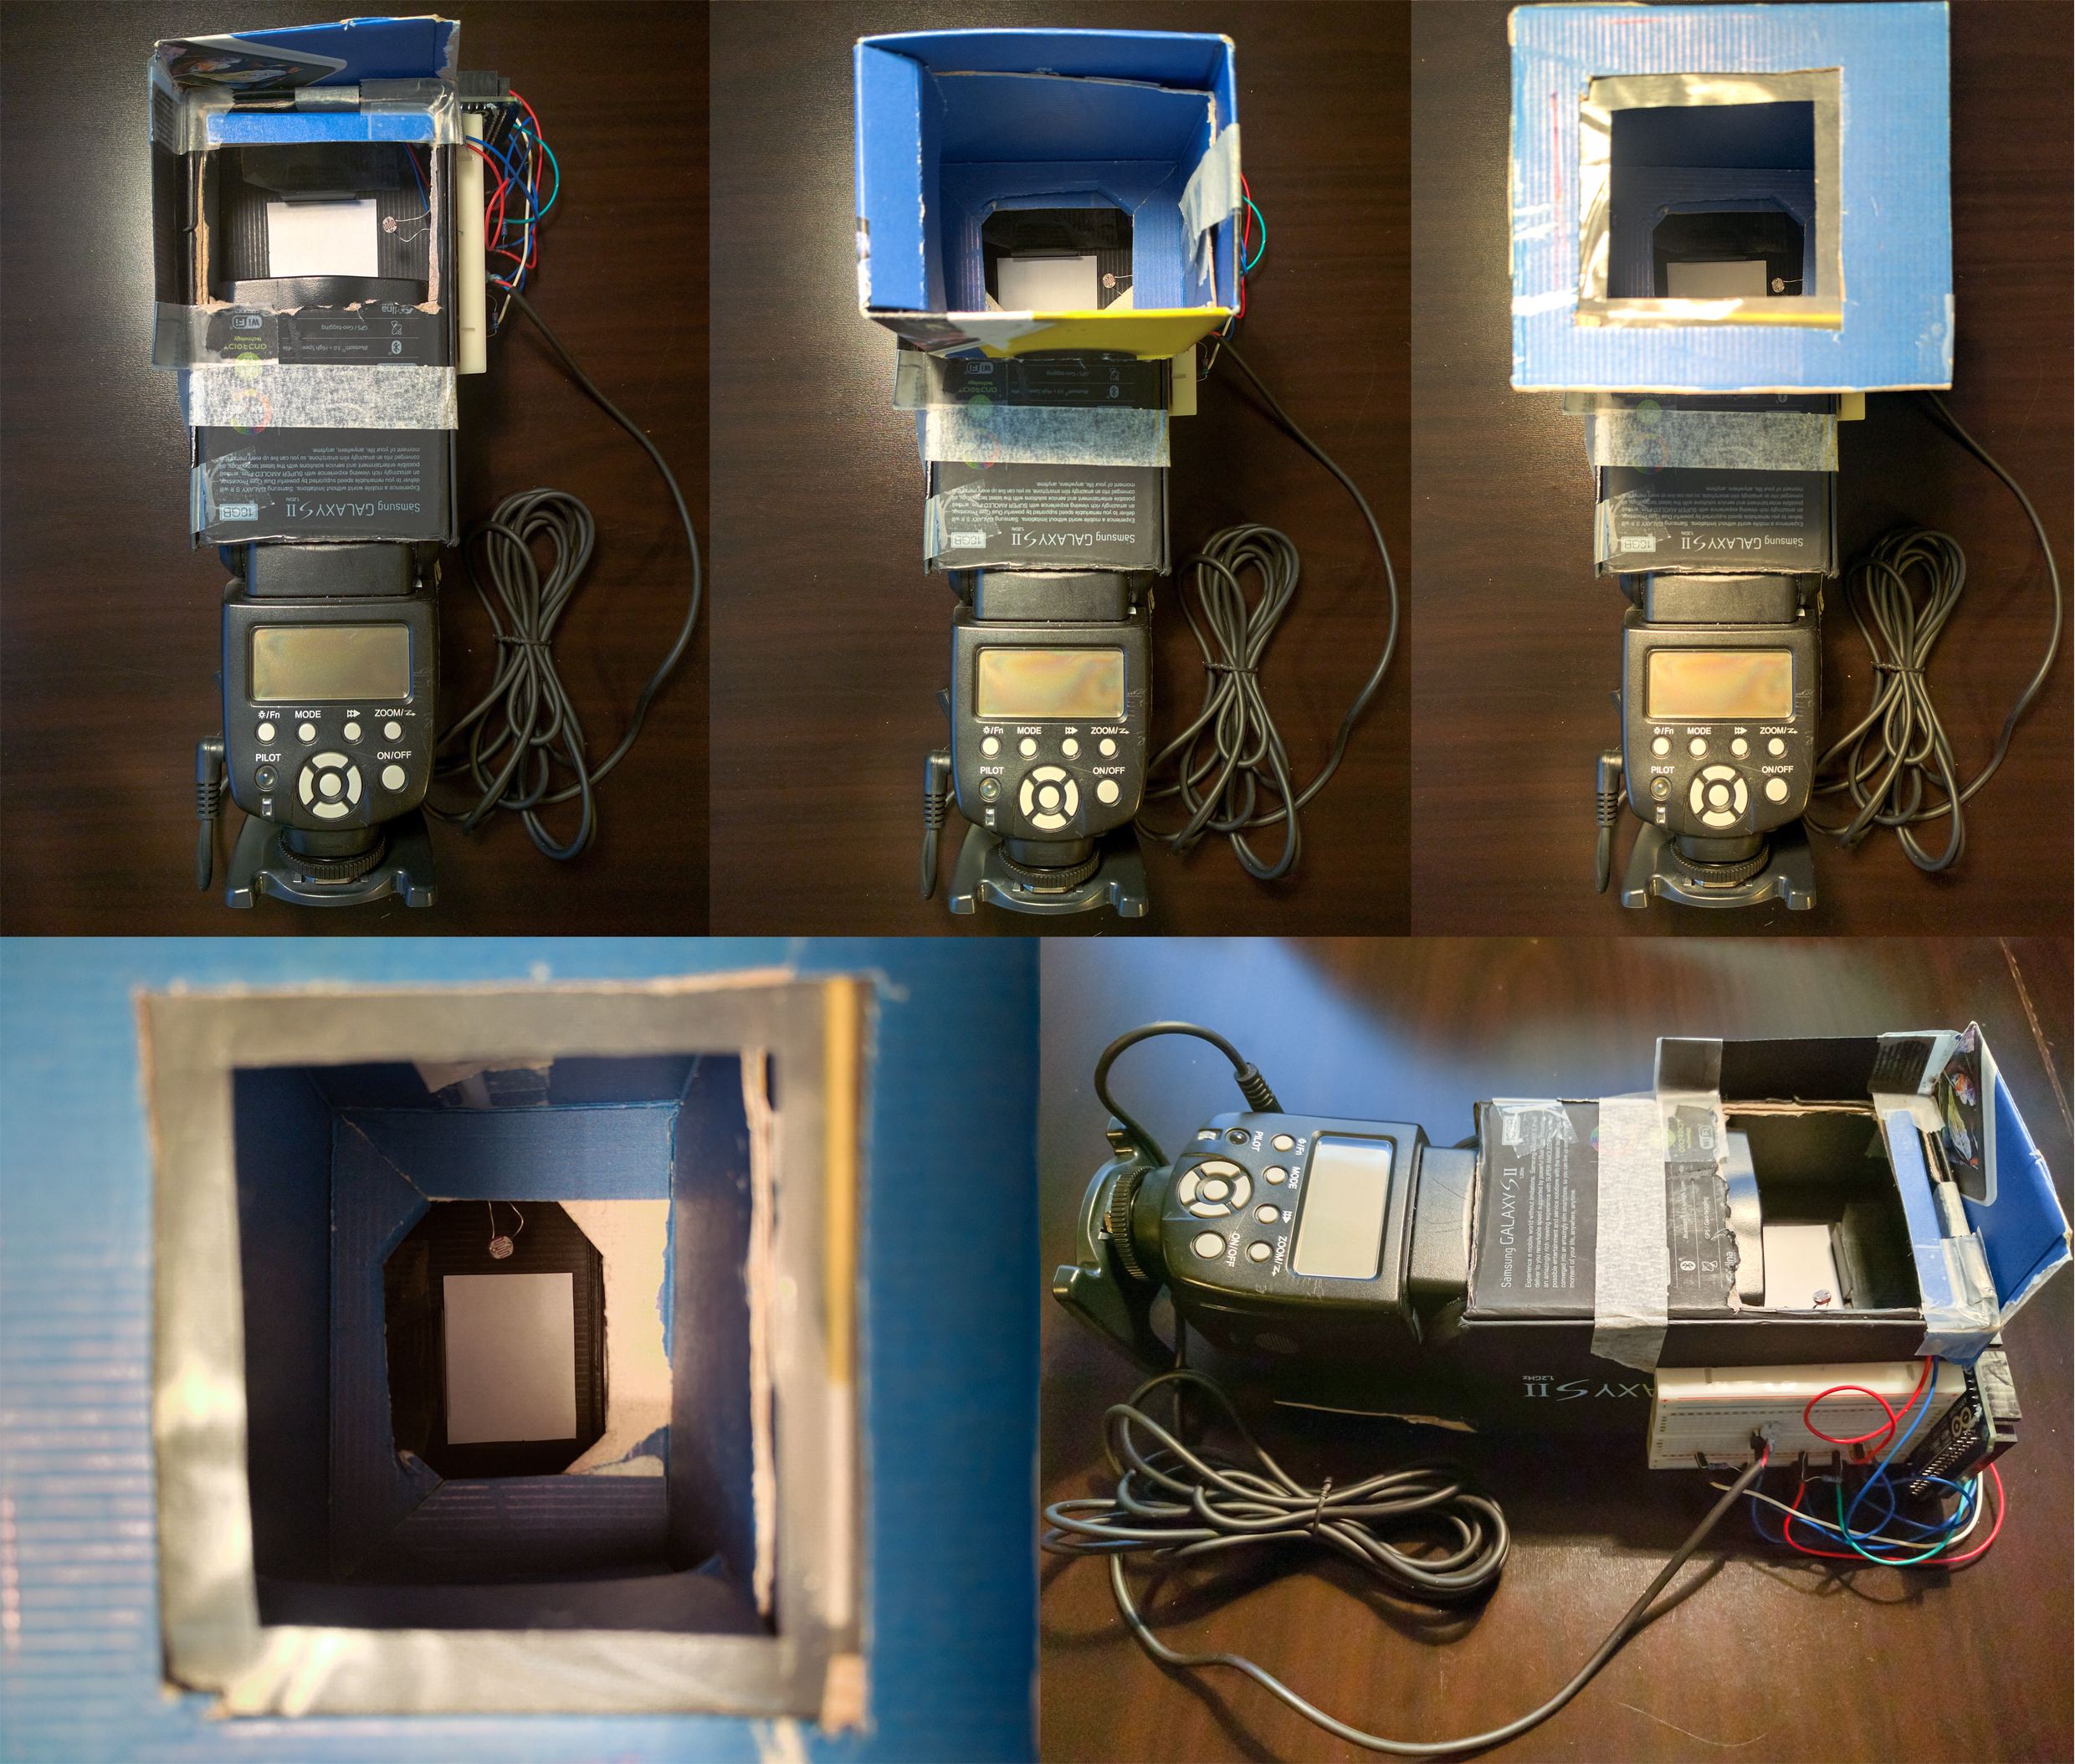
\includegraphics[width=\textwidth,height=\textheight,keepaspectratio=true]{images/design_implementation/camera_module-actual.jpg}
\end{figure}




\chapter{Microcontroller Schematics}
\label{appendix:camera-module-schematics}

The schematics for the external camera module featuring an Arduino Mega 2560 microcontroller. An optocoupler (4N35) is used to safely isolate the external light source from the rest of the circuit.

\begin{figure}[h]
\centering 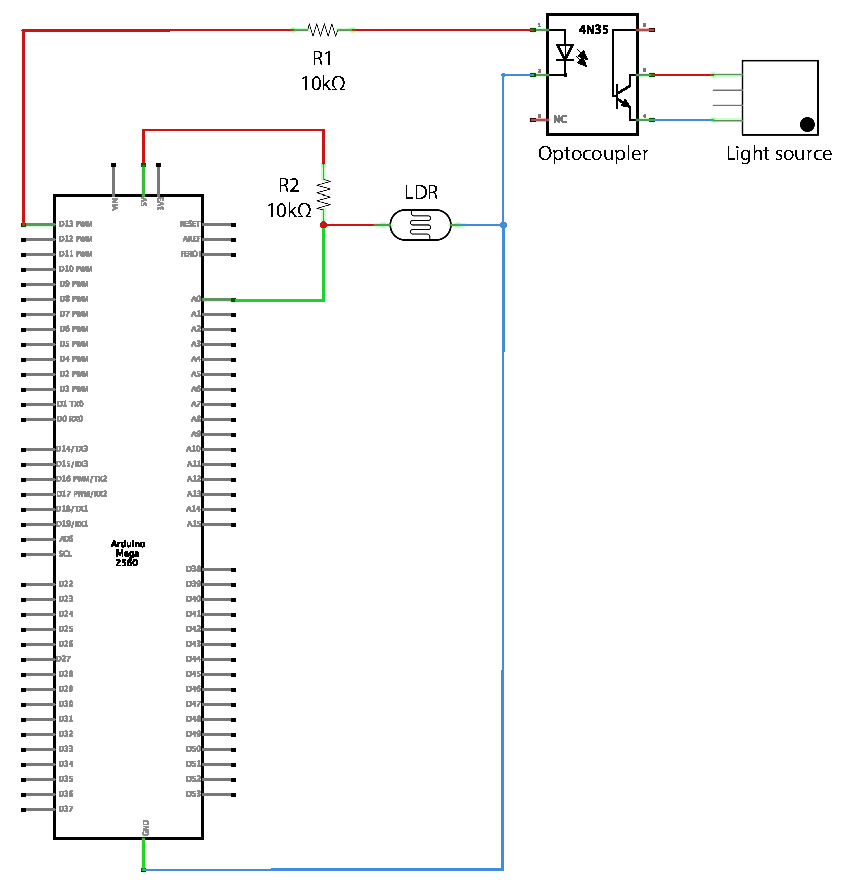
\includegraphics[width=12cm]{images/design_implementation/arduino_schematics.pdf}
\end{figure}





\chapter{Microcontroller Program (Arduino)}
\label{appendix:microcontroller-program}

The code utilizes Simon Monk's Arduino Timer library (version 1.3) \cite{arduino_timer_library}.

\lstinputlisting[language=C++,caption={main.ino}]{../app/camera-module/arduino/code/code.ino}
\clearpage
\lstinputlisting[language=C++,caption={is\_focused.ino}]{../app/camera-module/arduino/code/is_focused.ino}




\chapter{Fingerprint format}
\label{appendix:fingerprint}

The fingerprint can be represented as a $n \times m$ matrix where $n$ denotes the number of frames and $m$ the maximum number of peaks found in a single frame (sample), and encoded as a JavaScript array with additional metadata:
\[
M=
  \begin{bmatrix}
    P_{11} & P_{12} & P_{13} \\
    P_{21} & P_{22} & 0 \\
    P_{31} & 0 & 0
  \end{bmatrix}
\]
\begin{lstlisting}[language=json,firstnumber=1]
[
  {
    timestamp: 252,
    peaks: [
      { hue: 76, intensity: 770 },
      { hue: 90, intensity: 693 },
      { hue: 60, intensity: 301 }
    ]
  },
  {
    timestamp: 844,
    peaks: [
      { hue: 74, intensity: 672 },
      { hue: 60, intensity: 310 }
    ]
  },
  {
    timestamp: 1440,
    peaks: [
      { hue: 60, intensity: 466 },
      { hue: 71, intensity: 466 }
    ]
  }
]
\end{lstlisting}


\chapter{Fingerprint Design Document}
\label{appendix:fingerprint-design-doc}
A CouchDB design document used for creating an index keyed by the peak count and weighted hue average of the first sample of each fingerprint to allow fingerprints to be queried directly by peak count and average hue.
\vspace{5mm}

\lstinputlisting[language=JavaScript]{./chapters/design_doc.js}

\chapter{Experiment Taggants}
\label{appendix:taggants}

For each LumiNova\textregistered\ pigment (luminophore) a stock solution was created. The taggants were created by pipeting the stock solutions in increments of $50\mu l$ into intermediary solutions, from which $50\mu l$ would be pipeted onto a blank white carton to form the taggant. For example, taggant \emph{13VP} would require $200\mu l$ of stock solution ($50\mu l$ and $150\mu l$ of pigments G and O, respectively), of which $50\mu l$ would be pipeted on to the carton.
\vspace{-1em}
\begin{table}[ht]
  \caption{The amount of phosphor used for creating the stock solutions.}

  \begin{center}
  \begin{tabular}{| m{1.75cm} | c | c |}
    \hline
    \textbf{Pigment}  & \textbf{Phosphor (g)} & \textbf{Stock solution (ml)} \\ \hline
    O & 0,1416 & 1,42 \\
    \hline
    G & 0,1558 & 1,56 \\
    \hline
    DB & 0,1454 & 1,45 \\
    \hline
  \end{tabular}
  \end{center}
\end{table}
\vspace{-2.75em}
\begin{table}[ht]
  \caption{The pigment proportions for each taggant. The numbers indicate how many $50\mu l$ of the corresponding stock solution would be used in the intermediary solution used for creating the taggant.}

  \begin{center}
  \begin{tabular}{| m{1.75cm} | c | c | c |}
    \hline
    \textbf{Taggant}  & \textbf{Red (O)} & \textbf{Green (G)} & \textbf{Blue (DB)} \\ \hline
    S & -- & -- & 1 \\
    \hline
    P & 1 & -- & -- \\
    \hline
    13SP & 3 & -- & 1 \\
    \hline
    13VP & 3 & 1 & -- \\
    \hline
    13SV & -- & 3 & 1 \\
    \hline
    24SP & 4 & -- & 2 \\
    \hline
    24VP  & 4 & 2 & -- \\
    \hline
    24SV & -- & 4 & 2 \\
    \hline
  \end{tabular}
  \end{center}
\end{table}

\end{document}